\documentclass[a4paper]{article}
\usepackage{amssymb}
\usepackage{array}
\usepackage{amsmath}
\usepackage[affil-it]{authblk}
\usepackage[backend=bibtex,style=numeric]{biblatex}
\usepackage{graphicx}
\usepackage{geometry}
\geometry{margin=1.5cm, vmargin={0pt,1cm}}
\setlength{\topmargin}{-1cm}
\setlength{\paperheight}{29.7cm}
\setlength{\textheight}{25.3cm}

\addbibresource{citation.bib}

\begin{document}
% =================================================
\title{Report for Numerical Analysis programming homework \# 2}

\author{Chen Shuo 12231064
  \thanks{Email address: \texttt{shuo\_chen@zju.edu.cn}}}
\affil{(Electronic Science and Technology), Zhejiang University }


\date{Submitted time: \today}

\maketitle
% ============================================
\section*{A.}
There are classes used in this homework:

\subsection*{A-a Function}
A virtual class with a virtual operator \verb|()| with a \verb|double| input type and a \verb|double| output type, which represents the function value at input \verb|x|.
\subsection*{A-b Newton\_Interpolation}
A class represents a Newton interpolation polynomial, inherited from \verb|Function|, with members:
\begin{itemize}
  \item \verb|F| : the interpolated function
  \item \verb|interpolation_points| : points for interpolation
  \item \verb|function_values|: function values of interpolation points
  \item \verb|dd|: table of divided difference
\end{itemize}
It has two constructors, for different inputs:
\begin{itemize}
  \item \verb|interpolation_points| and \verb|function_values|.
  \item \verb|F| and \verb|interpolation_points|, then \verb|function_values| can be calculated one by one.               
\end{itemize}
Divided difference table is generated in the following way:
\begin{itemize}
  \item For the first column, \verb|dd[i][0]| is the value of $f(x_i)$.
  \item From the second column, we calculate \verb|dd[j][i]| by \verb|dd[j][i] = | \\
    \verb|(dd[j][i-1] - dd[j-1][i-1])/(interpolation_points[j] - interpolation_points[j-i])|
\end{itemize}
After completing divide difference table, we can calculate the function value of interpolation function at a given $x$:
$$
p(x) = \verb|dd[0][0]| + \sum \limits_{i=1}^n\verb|dd[i][i]|\prod \limits_{j = 0}^{i-1}(x-x_j)
$$
where $p$ represents Newton interpolation function.

\subsection*{A-c Hermite\_Interpolation}
A class represents a Hermite interpolation polynomial, inherited from \verb|Function|, with members:
\begin{itemize}
  \item \verb|interpolation_points|, \verb|function_values|, \verb|dd|: same as \verb|Newton_Interpolation|.
  \item \verb|order|: order of each interpolation point, 1: only function value, 2: function value and derivate, ...
  \item \verb|derivate_values|: derivate values of given points.
\end{itemize}
The constructor has the input with:
\begin{itemize}
  \item \verb|points|: distinct interpolation points
  \item \verb|order|, \verb|function_values| and \verb|derivate_values|
\end{itemize}
The way of calculating divide difference table is a little different with \verb|Newton_Interpolation|, since it has same interpolation points with derivate values of different orders.
\begin{itemize}
  \item For the item \verb|dd[j][i]|, we use values in \verb|derivrate_values| \\
  if $\verb|interpolation_points[j] - interpolation_points[j-i]| == 0$
\end{itemize}

\subsection*{A-d Bezier\_Curve}
A class represents Bezier curves, with members:
\begin{itemize}
  \item \verb|t_points|: interpolation of $t$
  \item \verb|interpolation_points|: interpolation of $(x,y)$
\end{itemize}
The constructor has the input with:
\begin{itemize}
  \item \verb|t_points| and \verb|interpolation_points|
\end{itemize}
The point at time $t$ in the curve can be calculated as:
\begin{itemize}
  \item Determine $i$, s.t. $t$ belongs to the $i$-th part of interval $[t_i,t_{i+1}]$
  \item According to the algorithm in the book, and use difference instead of derivate due to the difficulty in getting derivate, 
  calculate $\textbf{q}_j = \frac{j}{3}\textbf{p}_i + \frac{3-j}{3}\textbf{p}_{i+1}$, for $j = 0,1,2,3$
  \item $\textbf{B}(t) = \sum\limits_{k=0}^3{n\choose k}t^k(1-t)^{3-k}\textbf{q}_k$
\end{itemize}

\section*{B}
According to ProblemB, Figure \ref{fig:ProblemB} is plotted and Runge phenomenon can be observed.
\begin{figure}[h]
  \centering
  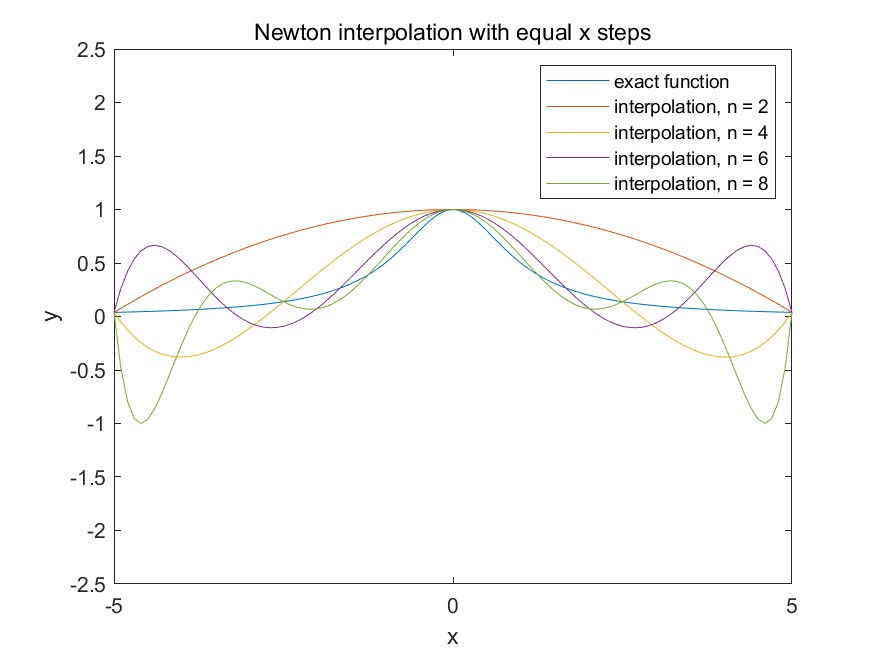
\includegraphics[width=0.4\textwidth]{fig/ProblemB.jpg}
  \caption{ProblemB}
  \label{fig:ProblemB}
\end{figure}

\section*{C}
According to ProblemC, Figure \ref{fig:ProblemC} is plotted using the zeros of Chebyshev polynomials.
It can be observed that Runge phenonmenon has been eliminated.
\begin{figure}[htbp]
  \centering
  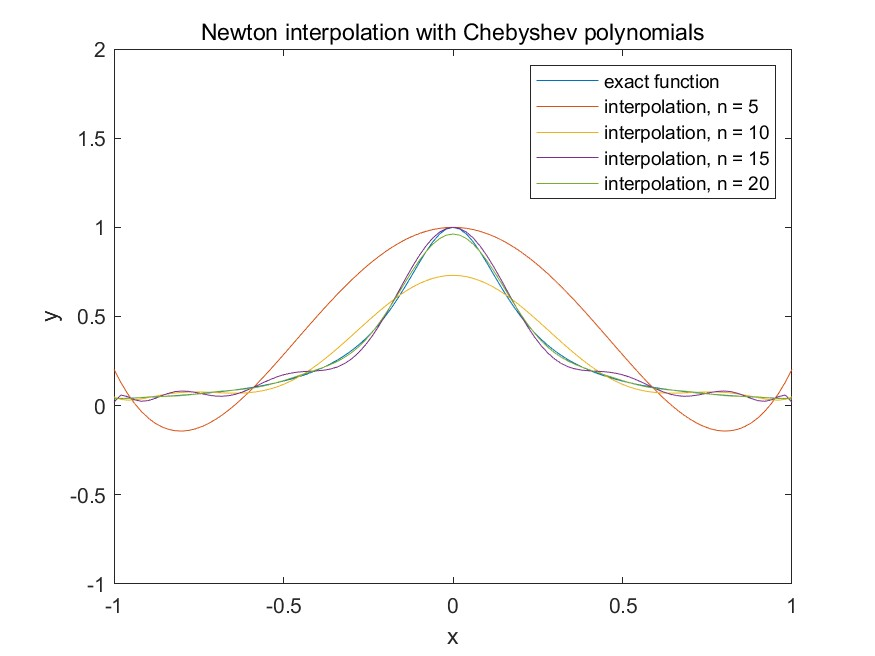
\includegraphics[width=0.4\textwidth]{fig/ProblemC.jpg}
  \caption{ProblemC}
  \label{fig:ProblemC}
\end{figure}

\section*{D}
\subsection*{D-a}
Using the subroutine in \verb|Interpolation.hpp|, we get a Hermite polynomial $p(t)$. The results are:
\begin{itemize}
  \item $p(10) = 742.503$
  \item $p'(10) = 48.382$
\end{itemize}
It means the position and speed is 742.503 and 48.382 respectively.
\subsection*{D-b}
Using $p(t)$ in D-a to examine whether its speed would exceed 81, and output the time if it does.
According to the result of \verb|ProblemD.cpp|, it speed exceeds 81 at $t=6$.

\section*{E}
\subsection*{E-a}
Using the subroutine in \verb|Interpolation.hpp|, we get two Newton interpolation polynomials $p_1(t)$, $p_2(t)$. The figure is plotted as follows:
\begin{figure}[htbp]
  \centering
  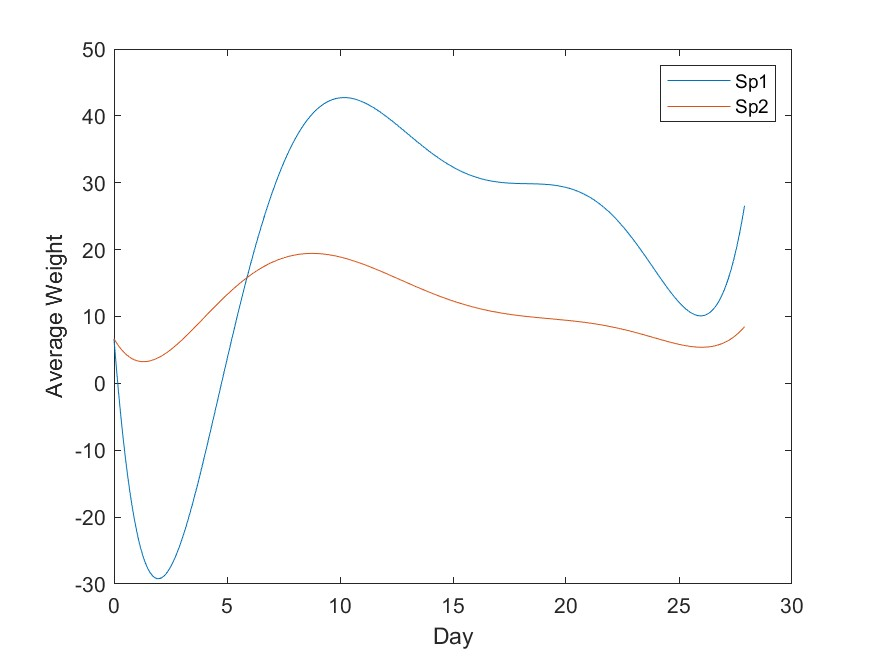
\includegraphics[width=0.4\textwidth]{fig/ProblemE.jpg}
  \caption{ProblemE}
  \label{fig:ProblemE}
\end{figure}
\subsection*{E-b}
Using $p_1(t)$, $p_2(t)$ in D-a to predict function values at $t=43$. According to the result of \verb|ProblemE.cpp|, 
the average weight of Sp1 and Sp1 are 14640 and 2981 respectively, and $p_i(t) > 0$ for $\forall t \in [28,43]$, $i = 1,2$, 
which means they both survive after another 15 days.

However, what needs to pay attention is that this result is not reliable for predicting the points out of the interpolation interval. Morever, even if 
for those points in the interpolation interval, it is either not reliable, for example, $p_1(t) < 0$ when $t$ is at about [1,5] according to Figure \ref{fig:ProblemE}, which is not reasonable.

\section*{F}
Using the subroutine in \verb|Interpolation.hpp|, we get a Bezier curve $\textbf{B}(t)$ by the following steps:
\begin{itemize}
  \item Get parametric equations of $x$ and $y$ of $t$: $x(t) = \sqrt{3}\sin(2\pi t)$, $y(t) = \frac{2}{3}(\sqrt{\sqrt{3}|\sin(2\pi t)|} + \sqrt{3} \cos(2\pi t))$
  \item Divide [0,1] into $m$ parts for interpolation of $t$, and calculate $(x_i,y_i)$ for each $t_i$
  \item Put all of $t_i$ and $(x_i,y_i)$ into the subroutine and get $\textbf{B}(t)$
  \item Change the value of $m$ and repeat the 2nd and 3rd steps
  \item Divide [0,1] into $N$ parts for sampling points to plot, here I choose $N=500$
\end{itemize}
Finally, the figure is plotted as follows:
\begin{figure}[htbp]
  \centering
  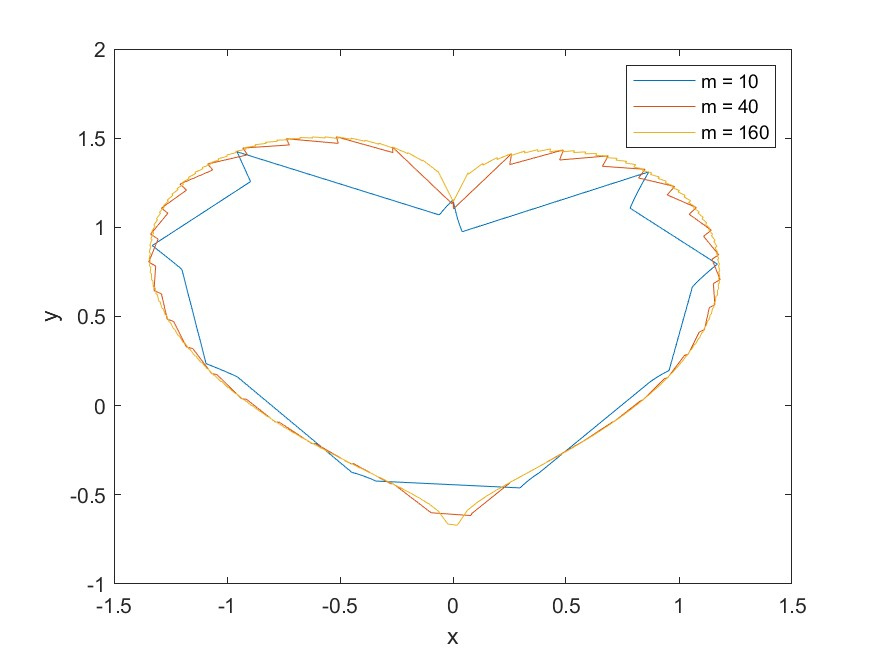
\includegraphics[width=0.6\textwidth]{fig/ProblemF.jpg}
  \caption{ProblemF}
  \label{fig:ProblemF}
\end{figure}




\end{document}


